We have chosen to follow an Agile software development approach, with weekly meetings to evaluate tasks. So far we have determined the architecture for our system and database (may be subject to minor changes in future iterations), and implemented the bare bones of server and client applications. 

Figure \ref{dbfig} below shows the structure of the database that is stored server side. 

\begin{figure}[h!]
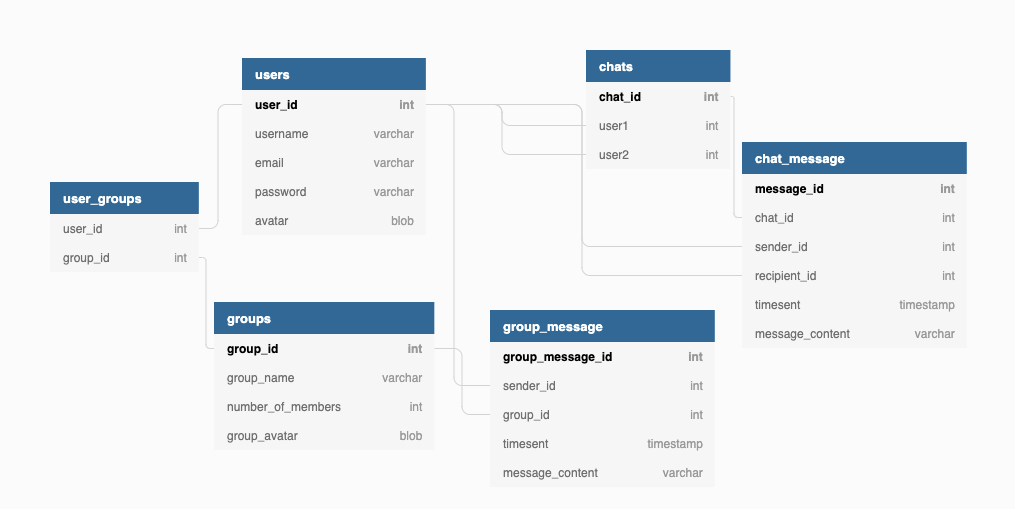
\includegraphics[width=\linewidth]{db.png}
\caption{Database structure}
\label{dbfig}
\end{figure}

\subsubsection{Web app} 

 The web app has been implemented with Vue.js for the UI, and javascript embeded inside html pages. The app has a RESTful server with SpringBoot that is responsible for mapping and routing. For individual clients to interact with the main application server, they fetch the web app from the RESTful web server, and then communicate with the main application server in JSON messages using javascript's web sockets. 

\subsubsection{Android app}

The Android application (developed using Java with XML for front-end layouts) has established a Websocket connection test to a remote dummy server and successfully sent and received JSON requests using an internally built JSON construction tool. The app has an SQLite local database attached used to store and retrieve previous client chats. Several functionalities are implemented (registration, login, sign out, unregister, sending messages) and need to be orchestrated with the server. There have been added unit tests for anti SQL injection input validation checks (using regex) alongside instrumented tests for internal tools check.

\subsubsection{Server} 

The main server, implemented in Java, can currently receive REGISTER, LOGIN, TEXT, and UNREGISTER requests from clients in a JSON format via a web socket. The server appropriately responds to these requests by creating a user in the PostgreSQL database, checking login details, sending the text message to the recipient user (storing for future retrieval if they are offline), or deleting the user from the database. 

\subsubsection{Deploying to Heroku}

We chose to use Heroku as a platform to deploy our server and database. So far, the database (in PostgreSQL) has been deployed to Heroku.

In the coming weeks we intend to deploy the application server as well so that full integration's tests can commence.